\section{Usage Scenario}\label{sec: usage_scenario}
We illustrate the use of HyperMap through a usage scenario where a journalist is collecting materials for a news story.
In~\autoref{sec: user_study}, we evaluate our system for conducting a literature review.
% We chose two different domains to demonstrate the flexibility of HyperMap.
% \subsection{Scenario 1: Collecting materials for a news story}
In this scenario, we use the \textit{All The News}~\cite{allthenews} dataset to demonstrate the effectiveness of HyperMap in assisting the exploration of the topics and keywords covered in news articles during a specific time period.
We randomly sampled 8192 news articles published in 2016 from the dataset for this case study.

Alice is a journalist currently working on a story about the US presidential election. She wants to collect articles about the 2016 election as materials for her story.
She can only vaguely remember certain events back when the election was happening, so she wants to freshen up her memory and find real evidence to reference.
Alice begins by opening the HyperMap system displaying the All The News dataset and searches `US presidential election'.
The Cluster View highlights relevant articles in each of the six topics with clear labels and colors (\autoref{fig: case_1}-a), and she can easily identify topics that are not related to the election. such as \textcolor{ride_hailing_technology}{`Ride-hailing Technology'}.
Before she filters the whole corpus with current search results, she wants to make sure that the relevancy threshold is reasonable so that she does not miss too many relevant articles.
The topic \textcolor{middle_east_threats}{`Security Threats in the Middle East'} caught her attention because she reckons that the seemingly unrelated topic might be related to the election since foreign policy towards the Middle East has always been a hot topic in the election.
She clicks on the topic label to highlight the topic and keywords.
She hovers over each of the highlighted keyword clusters, but she does not find any keywords related to the election.
Upon quickly scanning through the titles of the highlighted articles, she confirms that the topic is not related to the election and raises the threshold until the cluster is filtered out.

After that, she finds the remaining topics are too vague to tell what they are about. 
She decides to first drill down the topic \textcolor{controversies_and_challenges}{`Controversies and Challenges'} by clicking and expanding it (\autoref{fig: case_1}-b).
She finds that \textcolor{criminal_justice}{`Criminal Justice'} and \textcolor{political_protests}{`Political Protests against the Trump election'} are clearly two sub-topics that are related to the election.
Upon reading the summaries of the articles, she confirms the accuracy of these two sub-topic labels and marks them down.

After such an inspection, she is quite confident with the current relevancy threshold. 
She then clicks the `Filter Search' button to reorganize the corpus based on the search results (\autoref{fig: case_1}-c).
Once again, the topic \textcolor{concerns_and_controversies}{Concerns and Controversies in the United States} seems to contain a lot of related articles, but she could not tell what the topic is about.
To dive deeper, she splits the cluster into smaller, separated sub-clusters (\autoref{fig: case_1}-d).
The sub-clusters contain a wide range of topics, one of which being \textcolor{presidential_election_and_controversies}{`The 2016 US Presidential Election and Controversies'}.
Upon inspecting the mentioned keywords, she becomes curious about how `Vladimir Putin' is related to the election, so she clicks the keyword label to inspect the articles.
She also finds several interesting topics, such as \textcolor{presidential_eligibility}{`Presidential Eligibility Confusion'}.
She could not remember such controversies at first, but by browsing the highlighted keywords and reading the titles of the articles, she understands that it was a controversy between Donald Trump and Ted Cruz.
The wide range of topics brings her memory back, and she continues to click on every topic she deems relevant to the election to collect materials for her own story.

This case study demonstrates that HyperMap provides highly interpretable visualization of the topic structure and keyword connections in a corpus. 
Alice can quickly understand the topic if the labels are accurate, and she can always drill down to a deeper level to find more specific topics if the labels are too vague.
The keyword connections as well as article cards provide her with enough information to decide whether a topic is relevant to her story.
In the next case study, we demonstrate how the Analysis View can assist users in analyzing the selected documents.

\begin{figure}%
    \centering
    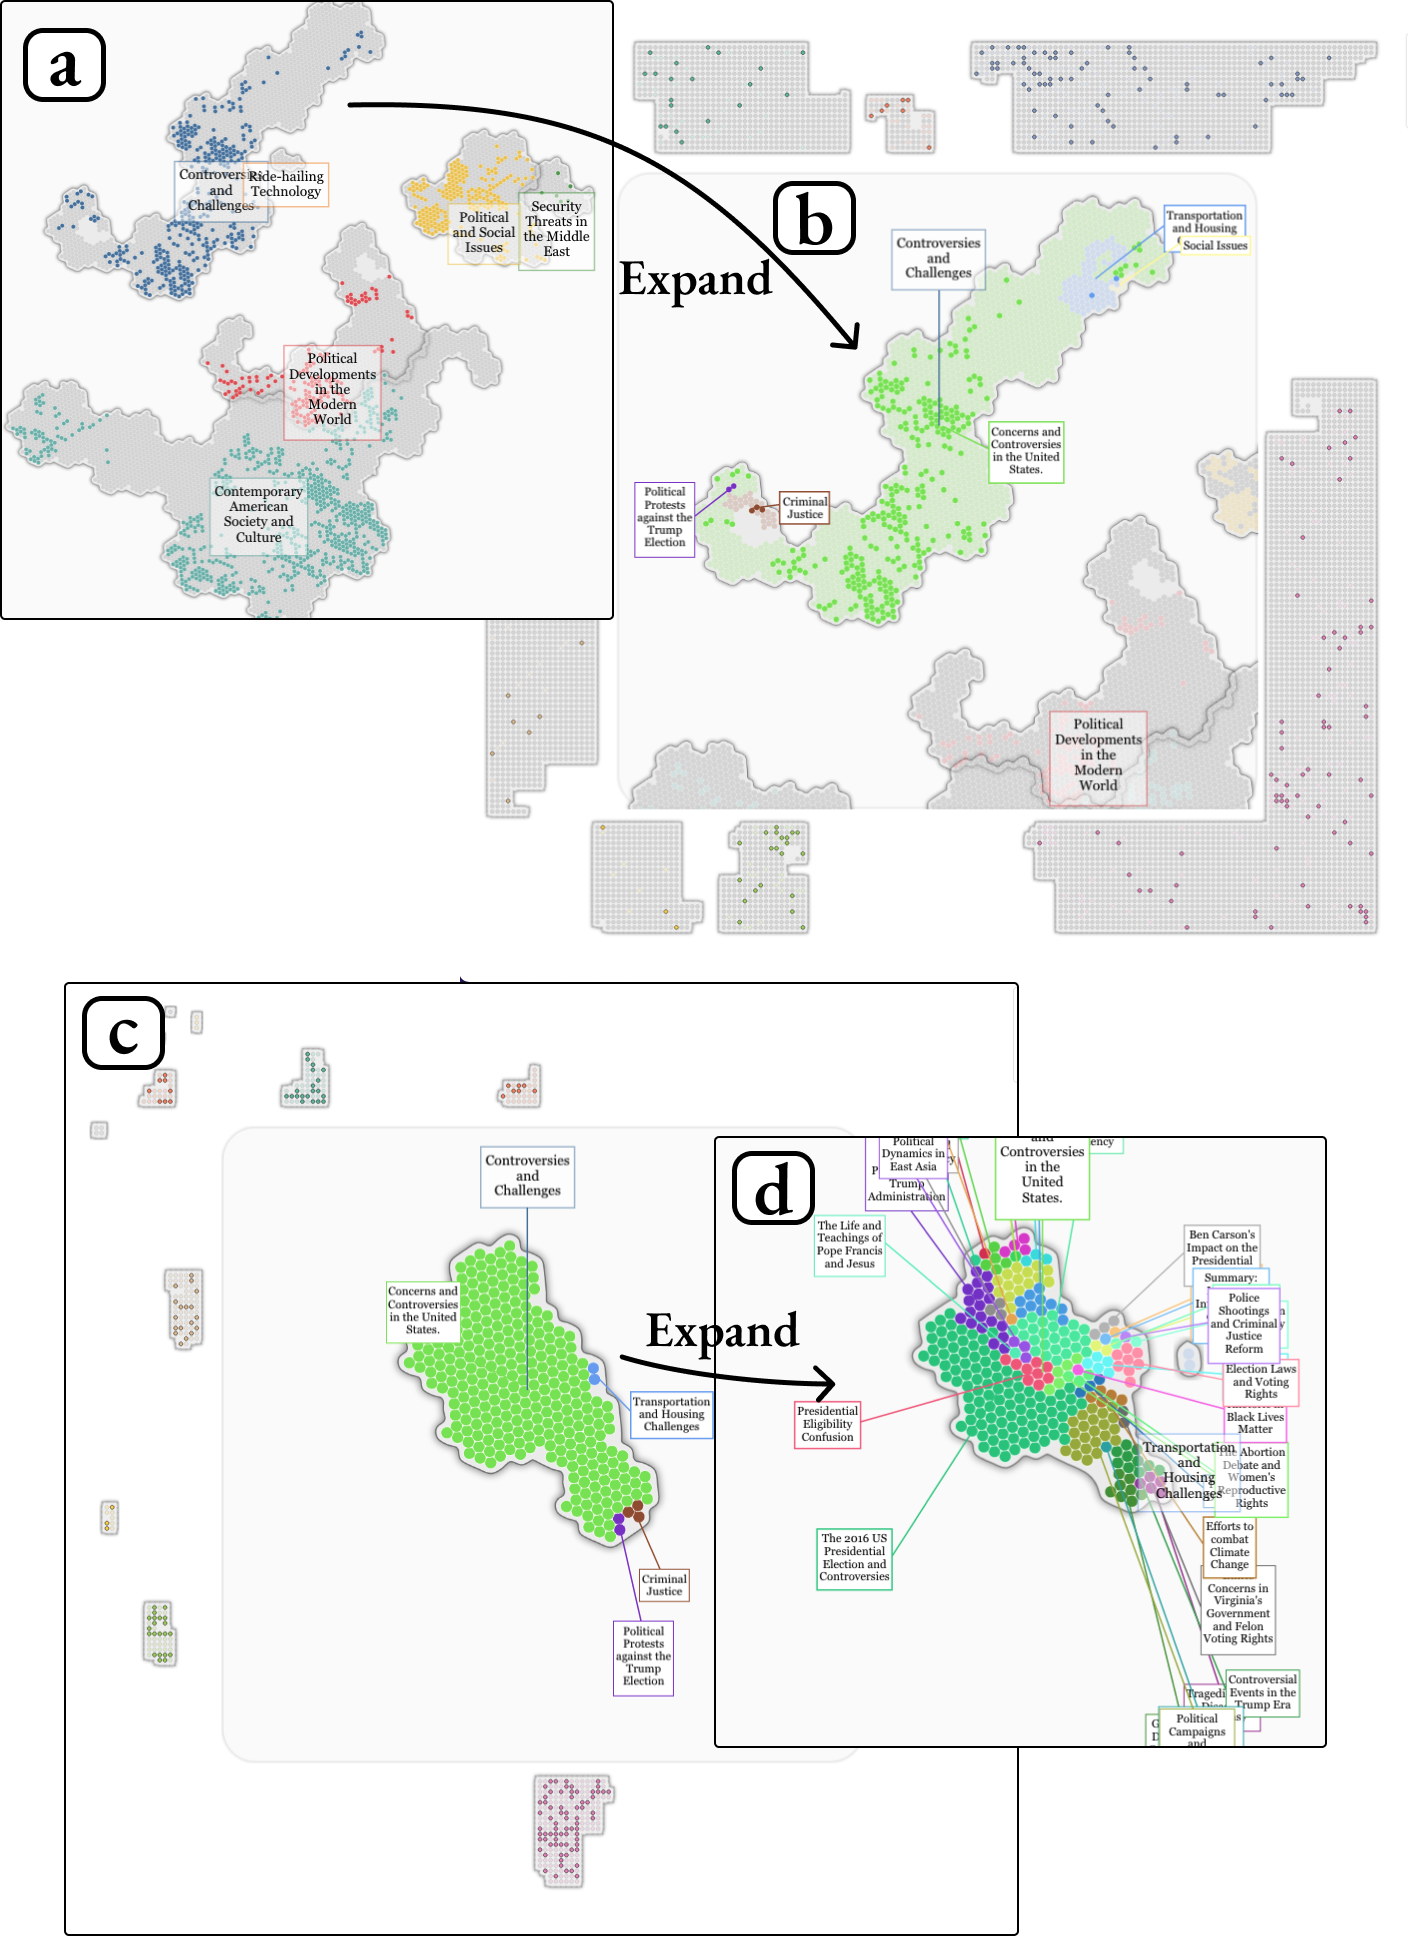
\includegraphics[keepaspectratio, width=\columnwidth]{case_1}
    \caption{User interactions in usage scenario 
    (a) The search result of `US presidential election'. Relevant articles are highlighted.
    (b) The user expands the topic `Controversies and Challenges', showing the sub-topics within and mentioned keywords in the peripheral area.
    (c) After clicking `Filter Search', irrelevant articles are removed, and the layout is regenerated.
    (d) The user expands a sub-topic `Concerns and Controversies in the United States'.
    }%
    \label{fig: case_1}%
\end{figure}
% TODO: figure~\autoref{fig: case_study_2}.
% \subsection{Scenario 2: Literature Review}
% In this usage scenario, we use the visualization publication dataset (VisPub)~\cite{vispub} to demonstrate how HyperMap can assist users in conducting literature research.
% % The prompts and responses are provided in supplemental materials.

% Bob is a Ph.D. student who is currently working on literature research in text analysis in visualization for his research project.
% Bob starts by loading the VisPub dataset into HyperMap. 
% Scanning through the topic structure, he can easily understand the topics like `Visualization of 3D Models, Volumes and Data', `Visualization of Medical Imaging and Blood Vessel Structures', and `Visualizations of Hierarchical Structures'.
% Since he is only interested in text visualization, he can quickly eliminate those clusters solely based on the topic labels.
% After a quick scan through all the topics presented, he proceeds to search `text analysis' and applies the filter.
% The search result shows that there are three related topics: `Visualization of Complex Data and Information Spaces', `Visualization of Web Data, Textual Data and Social Media Information', and `Visualization of Graphs and Networks'.
% From there, he starts to scan through each topic to decide if it should be included in his literature research.
% The mentioned keywords (author keywords) are particularly helpful in this process.
% They include data types, model names and visualization techniques, providing rich information about the topic.
% He can already get a gist of the research problems in text visualization, such as `Reasoning', `Topic Models' or `Temporal Patterns'.
% He finds those topics interesting, but not all of them are directly related to his research.
% By clicking on the keywords and roughly reading the abstracts, he can quickly decide whether to include it in his literature research. 
% He expands and eliminates topics until he is satisfied with the reorganization result (\autoref{fig: case_2}).
% After he feels confident about the overall picture, he starts to investigate the reorganized corpus in detail.

% First, he finds a rather general cluster \textcolor{vis_web_data}{`Visualization of Web Data, Textual Data \dots'} in the result, talking about the design space of text visualization.
% He selects the cluster, inserts the summaries to the prompt template, and prompts in the Analysis View: `Given the selected documents, what should I consider when designing text visualization?'.
% The chatbot responds with 10 bullet points, such as `Amount of text', `Placement of text' and `Customizability' while referencing the articles.
% The natural language explanation with references helps him quickly gain a basic understanding of the topic.
% He then proceeds to ask questions in more detail while inserting the full content, such as `What is considered a balanced ratio of text and charts?'.
% In the response, one key point that the chatbot emphasizes is that users are found to prefer charts with more textual annotations, as long as the placement of text is well-designed.
% By inserting the article, the chatbot is able to provide accurate answers tailored to the selected article, rather than replying generically.
% Bob continues this process by selecting other topics he is unfamiliar with and asking the chatbot questions.
% By the end, he is able to develop a clear understanding of the topics in text visualization and how researchers address them. 
% The complete chat history can be found in supplemental materials.

\begin{figure}%
    \centering
    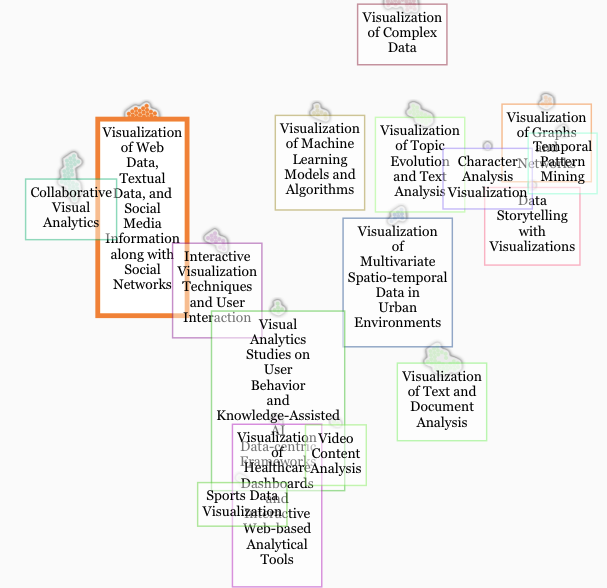
\includegraphics[keepaspectratio, width=\columnwidth]{case_2}
    \caption{
    The VisPub corpus visualization filtered by the keyword `text analysis' and reorganized by the user in usage scenario 2.
    After expansion and filtering, the remaining topics are at a reasonable level of granularity.
    The user is currently selecting the orange cluster `Visualization of Web Data, Textual Data and Social Media Information' to prompt the Analysis View for more detail.
    }%
    \label{fig: case_2}%
\end{figure}


